%%% title atcm2024
\documentclass[landscape,10pt]{jarticle}
\usepackage{pict2e}
\usepackage{ketpic2e,ketlayer2e}
\special{papersize=\the\paperwidth,\the\paperheight}
\usepackage{ketslide}
\usepackage{amsmath,amssymb}
\usepackage{bm,enumerate}
\usepackage[dvipdfmx]{graphicx}
\usepackage{color}
\usepackage[dvipdfmx,colorlinks=true,linkcolor=blue,filecolor=blue]{hyperref}

\def\deg#1{#1^{\circ}}
\newcommand{\monthday}{0627}
\renewcommand{\baselinestretch}{1.5}

\definecolor{slidecolora}{cmyk}{0.98,0.13,0,0.43}
\definecolor{slidecolorb}{cmyk}{0.2,0,0,0}
\definecolor{slidecolorc}{cmyk}{0.2,0,0,0}
\definecolor{slidecolord}{cmyk}{0.2,0,0,0}
\definecolor{slidecolore}{cmyk}{0,0,0,0.5}
\definecolor{slidecolorf}{cmyk}{0,0,0,0.5}
\definecolor{slidecolori}{cmyk}{0.98,0.13,0,0.43}
\def\setthin#1{\def\thin{#1}}
\setthin{0.1}
\newcounter{pagectr}
\setcounter{pagectr}{1}
\newcommand{\slidepage}[1][\monthday-]{%
\setcounter{ketpicctra}{18}%

\begin{layer}{118}{0}
\putnotew{130}{-\theketpicctra.05}{\small#1\thepage/\pageref{pageend}}
\end{layer}

}

\setmargin{23}{147}{10}{105}

\ketslideinit

\pagestyle{empty}

\begin{document}

\begin{layer}{120}{0}
\putnotese{0}{0}{{\Large\bf
\color[cmyk]{1,1,0,0}

\begin{layer}{120}{0}
{\Huge \putnotes{64}{15}{\LARGE {Development of methods for interactive classes}}}
\putnotes{62}{27}{\LARGE {using KeTLMS}}
\putnotes{62}{68}{Koji Nishiura, Setsuo Takato}
\putnotee{70}{87}{2024.12.10 ATCM2024}
\end{layer}

}
}
\end{layer}

\def\mainslidetitley{22}
\def\ketcletter{slidecolora}
\def\ketcbox{slidecolorb}
\def\ketdbox{slidecolorc}
\def\ketcframe{slidecolord}
\def\ketcshadow{slidecolore}
\def\ketdshadow{slidecolorf}
\def\slidetitlex{0}
\def\slidetitlesize{1.3}
\def\mketcletter{slidecolori}
\def\mketcbox{yellow}
\def\mketdbox{yellow}
\def\mketcframe{yellow}
\def\mslidetitlex{62}
\def\mslidetitlesize{2}

\color{black}
\Large\bf\boldmath
\addtocounter{page}{-1}

%%%%%%%%%%%%%

%%%%%%%%%%%%%%%%%%%%

\newslide{Contents of this talk}

\vspace*{18mm}

\textinit
\settext{3}{9}{130}

\begin{layer}{120}{0}
\addtext{8}{\ten}{Purpose of this research}
\end{layer}

%%%%%%%%%%%%%

%%%%%%%%%%%%%%%%%%%%


\sameslide

\vspace*{18mm}

\textinit
\settext{3}{9}{130}

\begin{layer}{120}{0}
\addtext{8}{\ten}{Purpose of this research}
\addtext[3]{8}{\ten}{KeTLMS}
\end{layer}


\sameslide

\vspace*{18mm}

\textinit
\settext{3}{9}{130}

\begin{layer}{120}{0}
\addtext{8}{\ten}{Purpose of this research}
\addtext[3]{8}{\ten}{KeTLMS}
\addtext[3]{8}{\ten}{Making teaching materials by KeTLMS}
\end{layer}


\sameslide

\vspace*{18mm}

\textinit
\settext{3}{9}{130}

\begin{layer}{120}{0}
\addtext{8}{\ten}{Purpose of this research}
\addtext[3]{8}{\ten}{KeTLMS}
\addtext[3]{8}{\ten}{Making teaching materials by KeTLMS}
\addtext[3]{8}{\ten}{Teaching materials}
\end{layer}


\sameslide

\vspace*{18mm}

\textinit
\settext{3}{9}{130}

\begin{layer}{120}{0}
\addtext{8}{\ten}{Purpose of this research}
\addtext[3]{8}{\ten}{KeTLMS}
\addtext[3]{8}{\ten}{Making teaching materials by KeTLMS}
\addtext[3]{8}{\ten}{Teaching materials}
\addtext[3]{8}{\ten}{Concluding remarks}
\end{layer}


\newslide{Purpose of this research}

\vspace*{18mm}

\textinit
\settext{6}{10}{115}

\begin{layer}{120}{0}
\addtext{1}{}{We are developing an LMS called KeTLMS.
Using KeTLMS, we will create teaching methods that allow us to objectively assess students' levels of understanding while conducting the class, based on verification of its educational effectiveness.}
\end{layer}

%%%%%%%%%%%%%

%%%%%%%%%%%%%%%%%%%%

\newslide{KeTLMS}

\vspace*{18mm}

\textinit
\settext{5}{10}{118}

\begin{layer}{120}{0}
\addtext{1}{}{KeTLMS is a system designed to streamline the process of teachers creating and distributing questions, while students receive the questions and submit their answers.
Additionally, it allows teachers to collect and grade the answers efficiently. }
\end{layer}

%%%%%%%%%%%%%

%%%%%%%%%%%%%%%%%%%%

\newslide{KeTLMS}

\vspace*{18mm}

\textinit
\settext{3}{10}{118}

\begin{layer}{120}{0}
\putnotese{5}{-5}{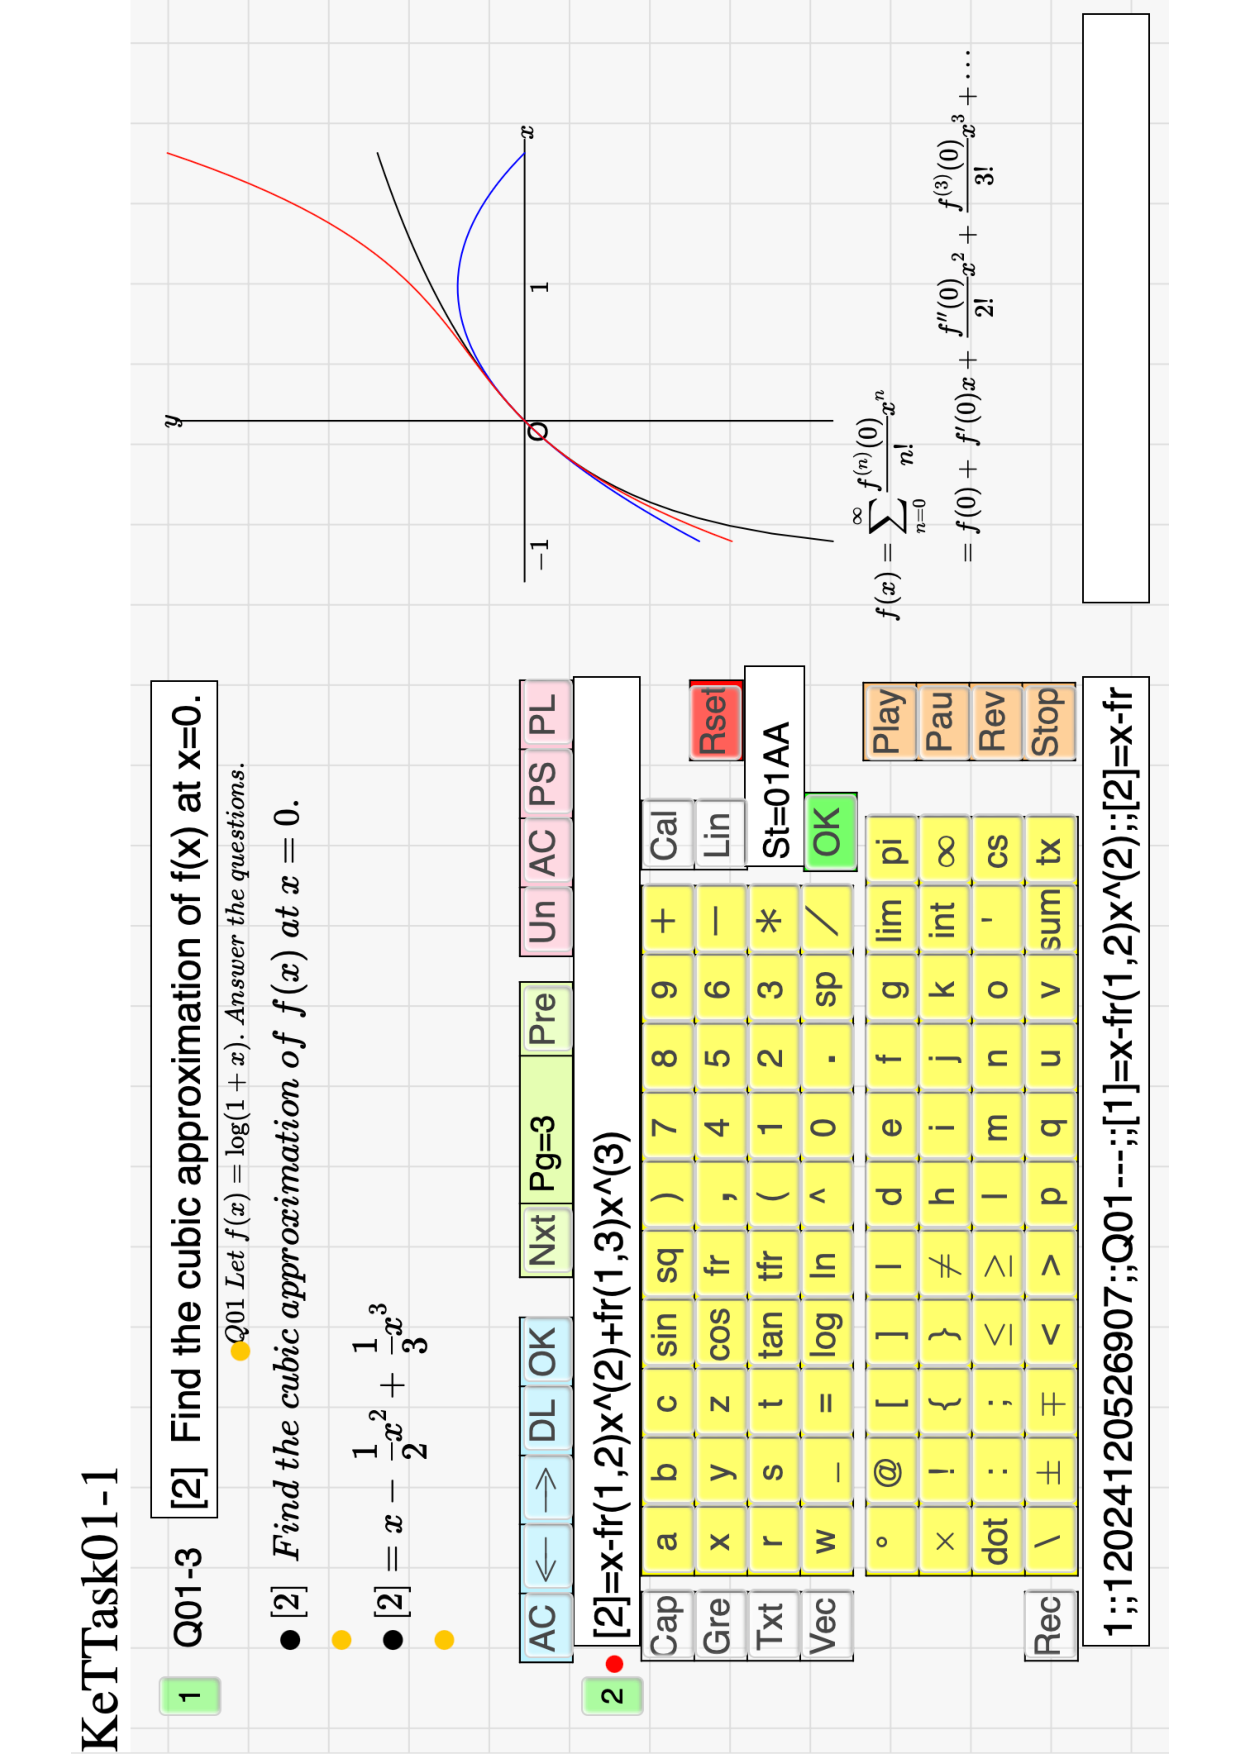
\includegraphics[bb=0.00 0.00 595.00 842.00,width=7cm,angle=-90]{fig/KeTTask01.pdf}}
\addtext[61]{0}{}{An important feature of the system is \vspace{-3mm}that both questions and answers are formatted as \vspace{-3mm}a single line of text.}
\end{layer}

%%%%%%%%%%%%%

%%%%%%%%%%%%%%%%%%%%

\newslide{Making \hspace{-0.3mm}teaching \hspace{-0.3mm}materials \hspace{-0.3mm}by \hspace{-0.3mm}KeTLMS}

\vspace*{18mm}

\textinit
\settext{6}{9}{130}

\begin{layer}{120}{0}
\putnotese{10}{1}{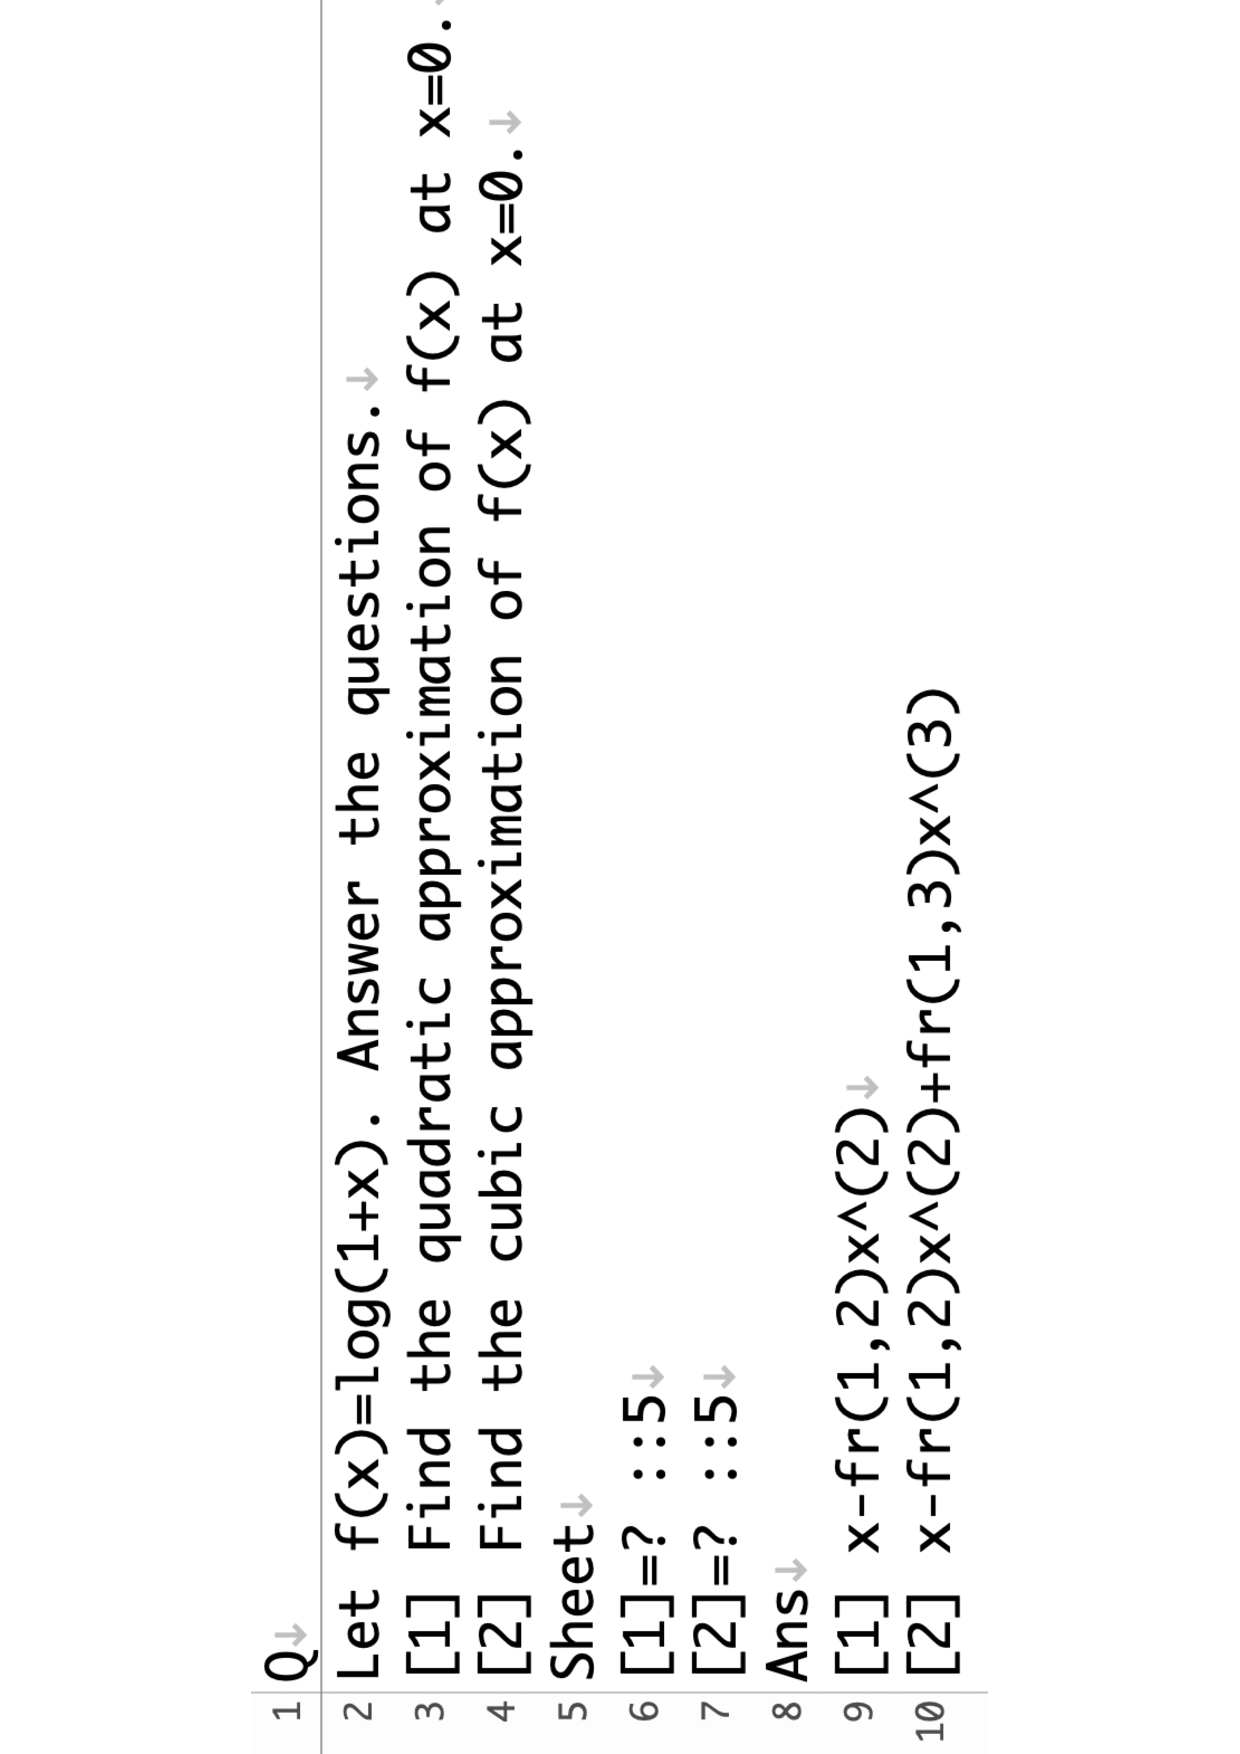
\includegraphics[bb=0.00 0.00 595.00 842.00,width=7cm,angle=-90]{fig/question01.pdf}}
\addtext{3}{1.}{Create a question file, `question01-1.txt'.}
\end{layer}

%%%%%%%%%%%%%

%%%%%%%%%%%%%%%%%%%%

\newslide{Making \hspace{-0.3mm}teaching \hspace{-0.3mm}materials \hspace{-0.3mm}by \hspace{-0.3mm}KeTLMS}

\vspace*{18mm}

\textinit
\settext{6}{9}{130}

\begin{layer}{120}{0}
\putnotese{6}{22}{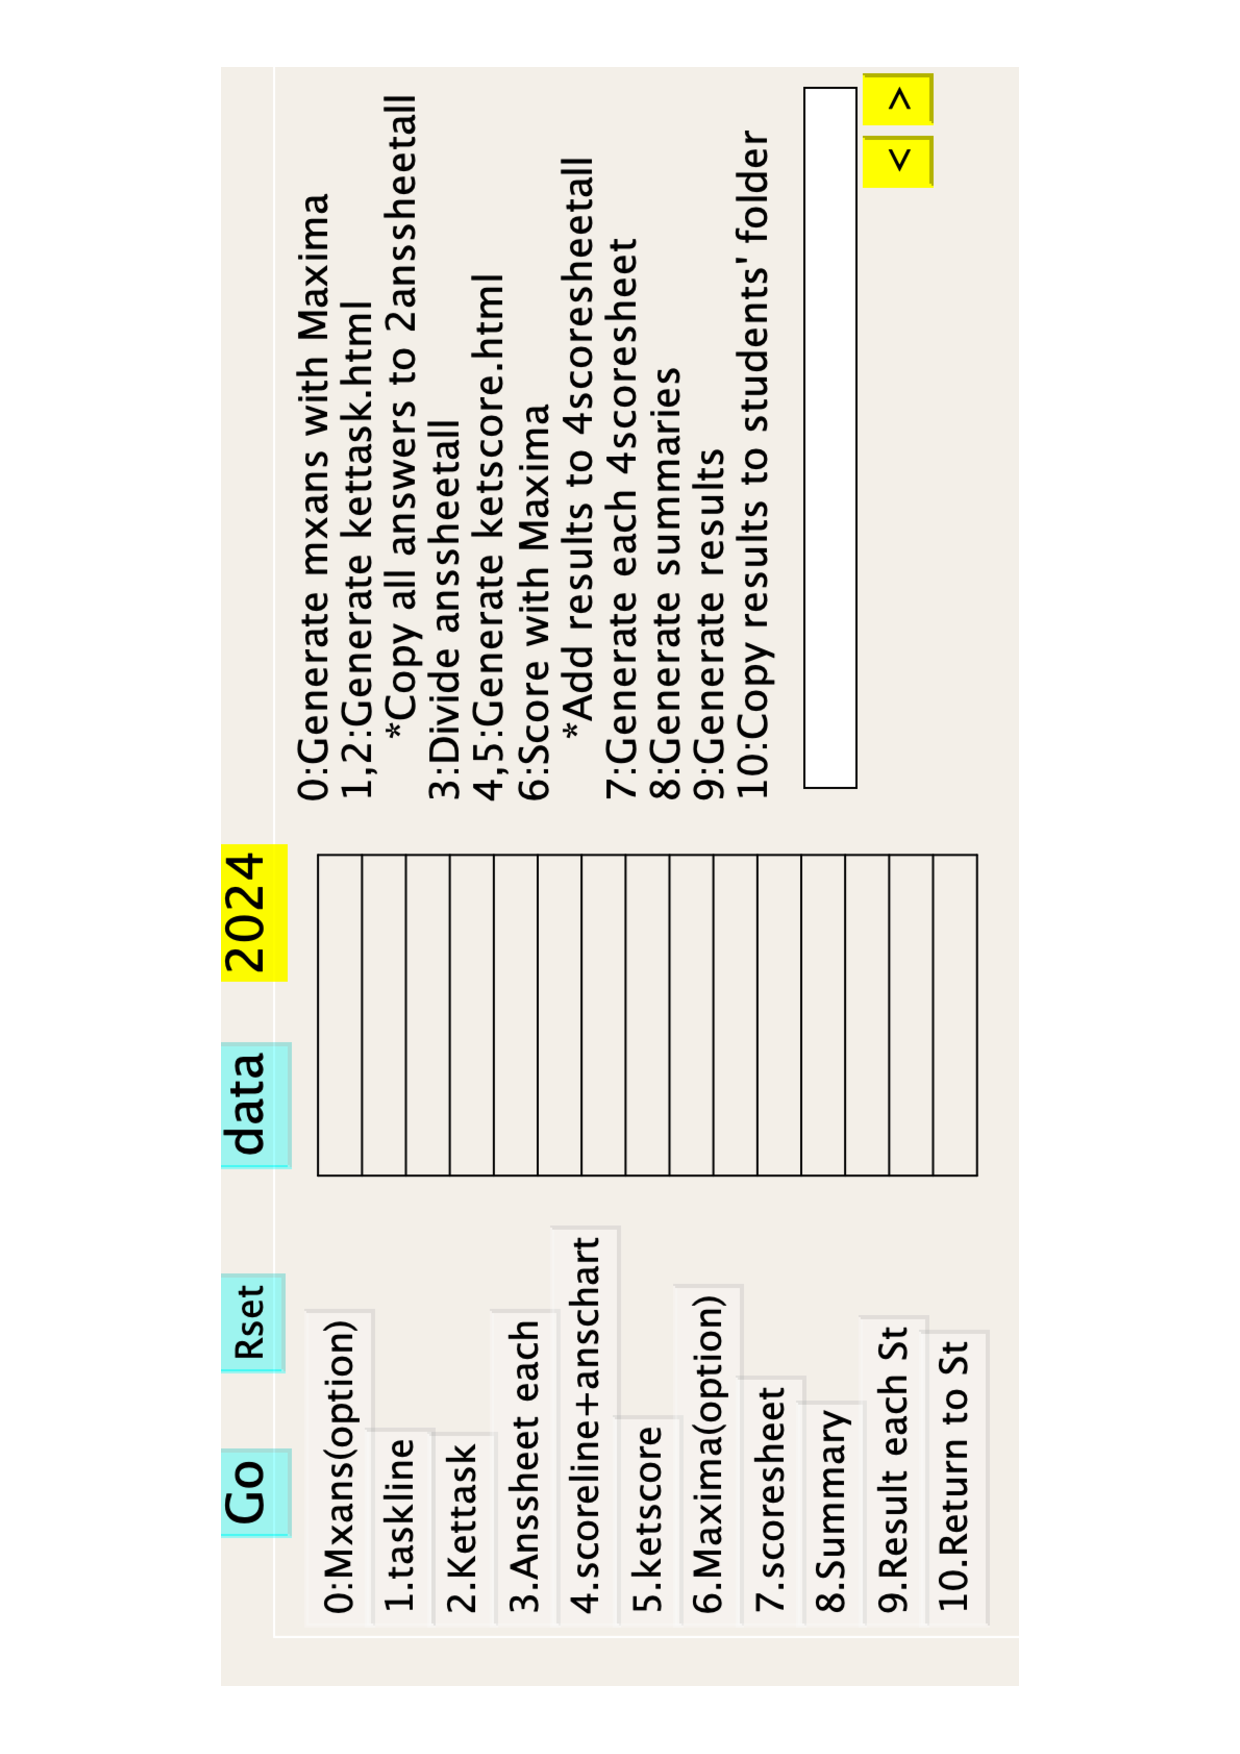
\includegraphics[bb=0.00 0.00 595.00 842.00,width=7cm,angle=-90]{fig/toolketmath.pdf}}
\addtext{3}{2.}{Create a question file, `kettaskv01-1E.html' }
\addtext{8}{}{by pressing bottuns `1.taskline' and `2.Kettask' }
\addtext{8}{}{in `toolketmathE.cdy'.}
\end{layer}

%%%%%%%%%%%%%

%%%%%%%%%%%%%%%%%%%%

\newslide{Making \hspace{-0.3mm}teaching \hspace{-0.3mm}materials \hspace{-0.3mm}by \hspace{-0.3mm}KeTLMS}

\vspace*{18mm}

\textinit
\settext{6}{9}{130}

\begin{layer}{120}{0}
\putnotese{5}{13}{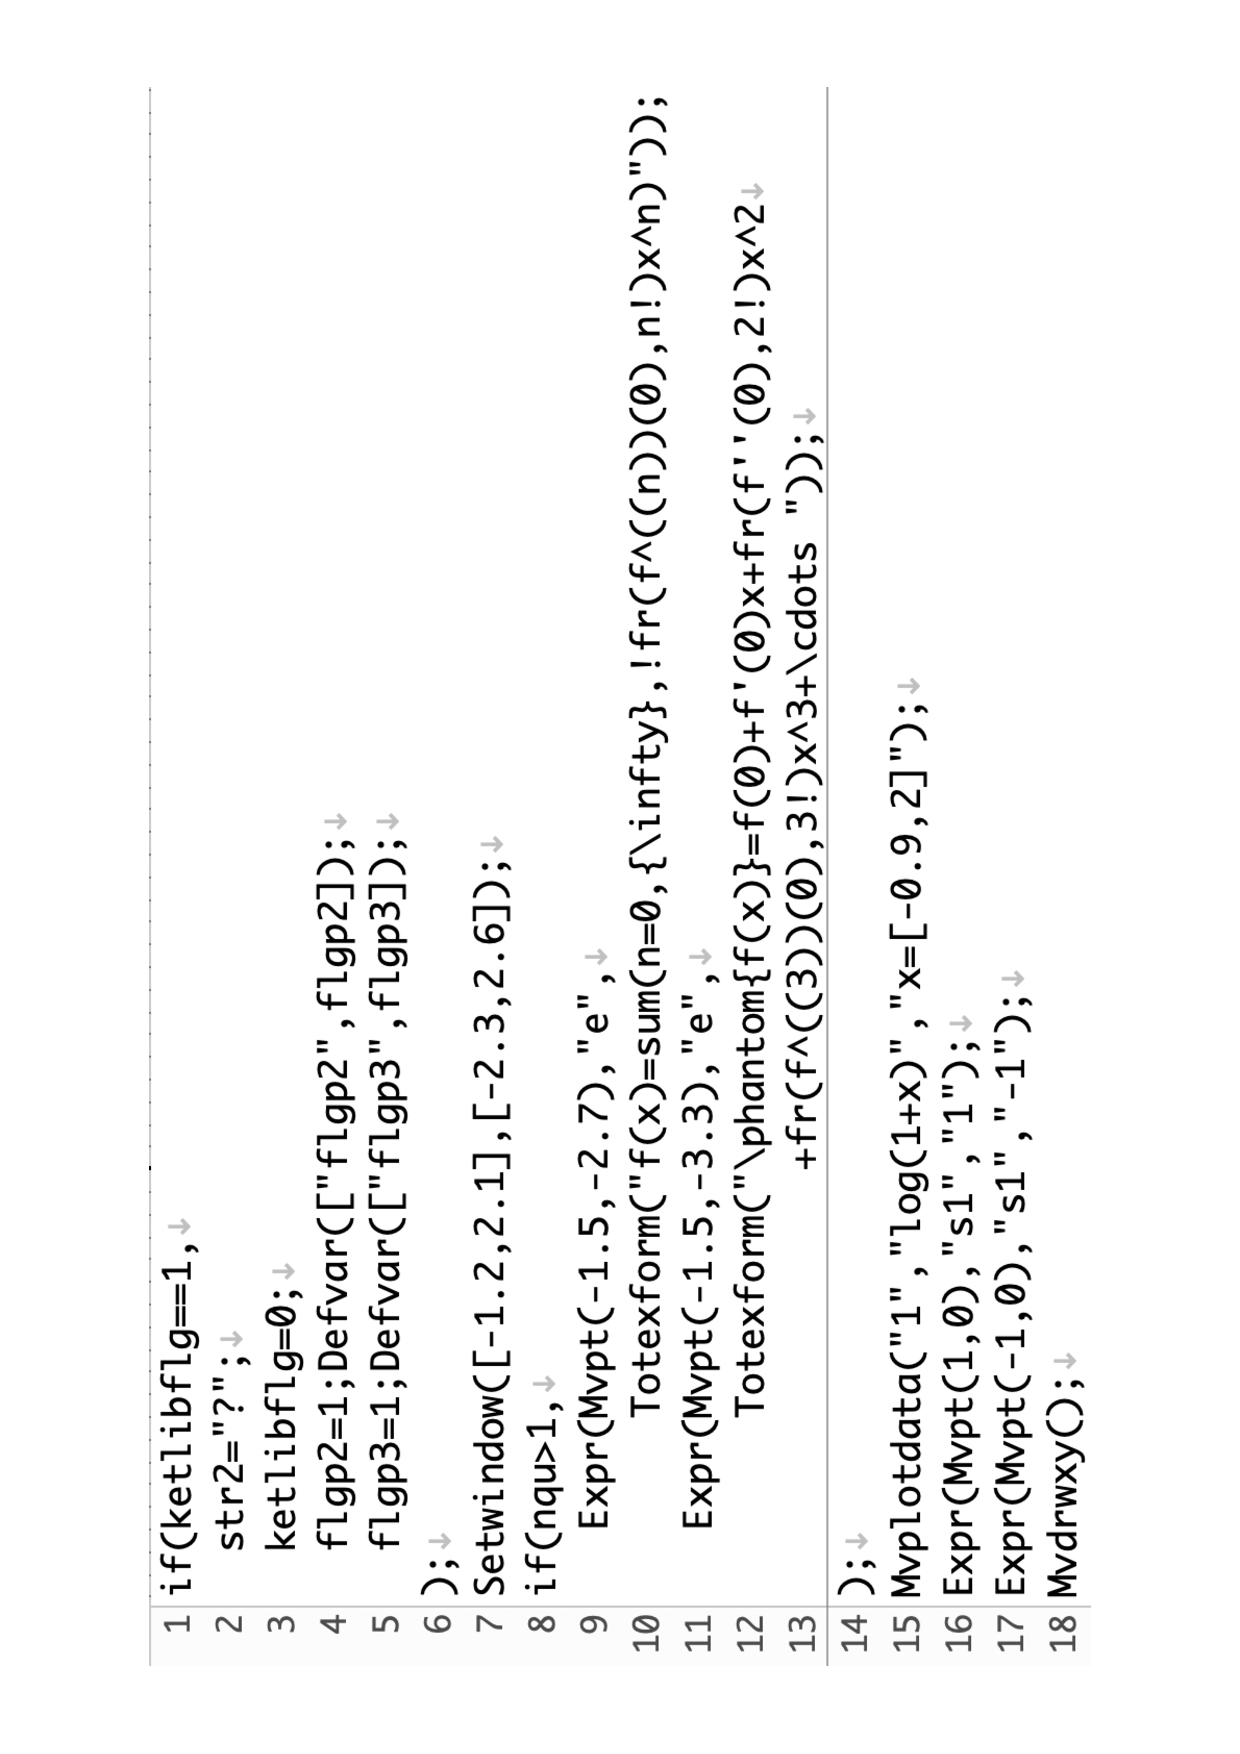
\includegraphics[bb=0.00 0.00 595.00 842.00,width=8cm,angle=-90]{fig/embedded_file.pdf}}
\addtext{3}{3.}{Create a file to embed in `kettaskv01-1E.html`,}
\addtext{8}{}{`001-1draw.txt'.}
\end{layer}

%%%%%%%%%%%%%

%%%%%%%%%%%%%%%%%%%%

\newslide{Making \hspace{-0.3mm}teaching \hspace{-0.3mm}materials \hspace{-0.3mm}by \hspace{-0.3mm}KeTLMS}

\vspace*{18mm}

\textinit
\settext{6}{9}{130}

\begin{layer}{120}{0}
\putnotese{10}{18}{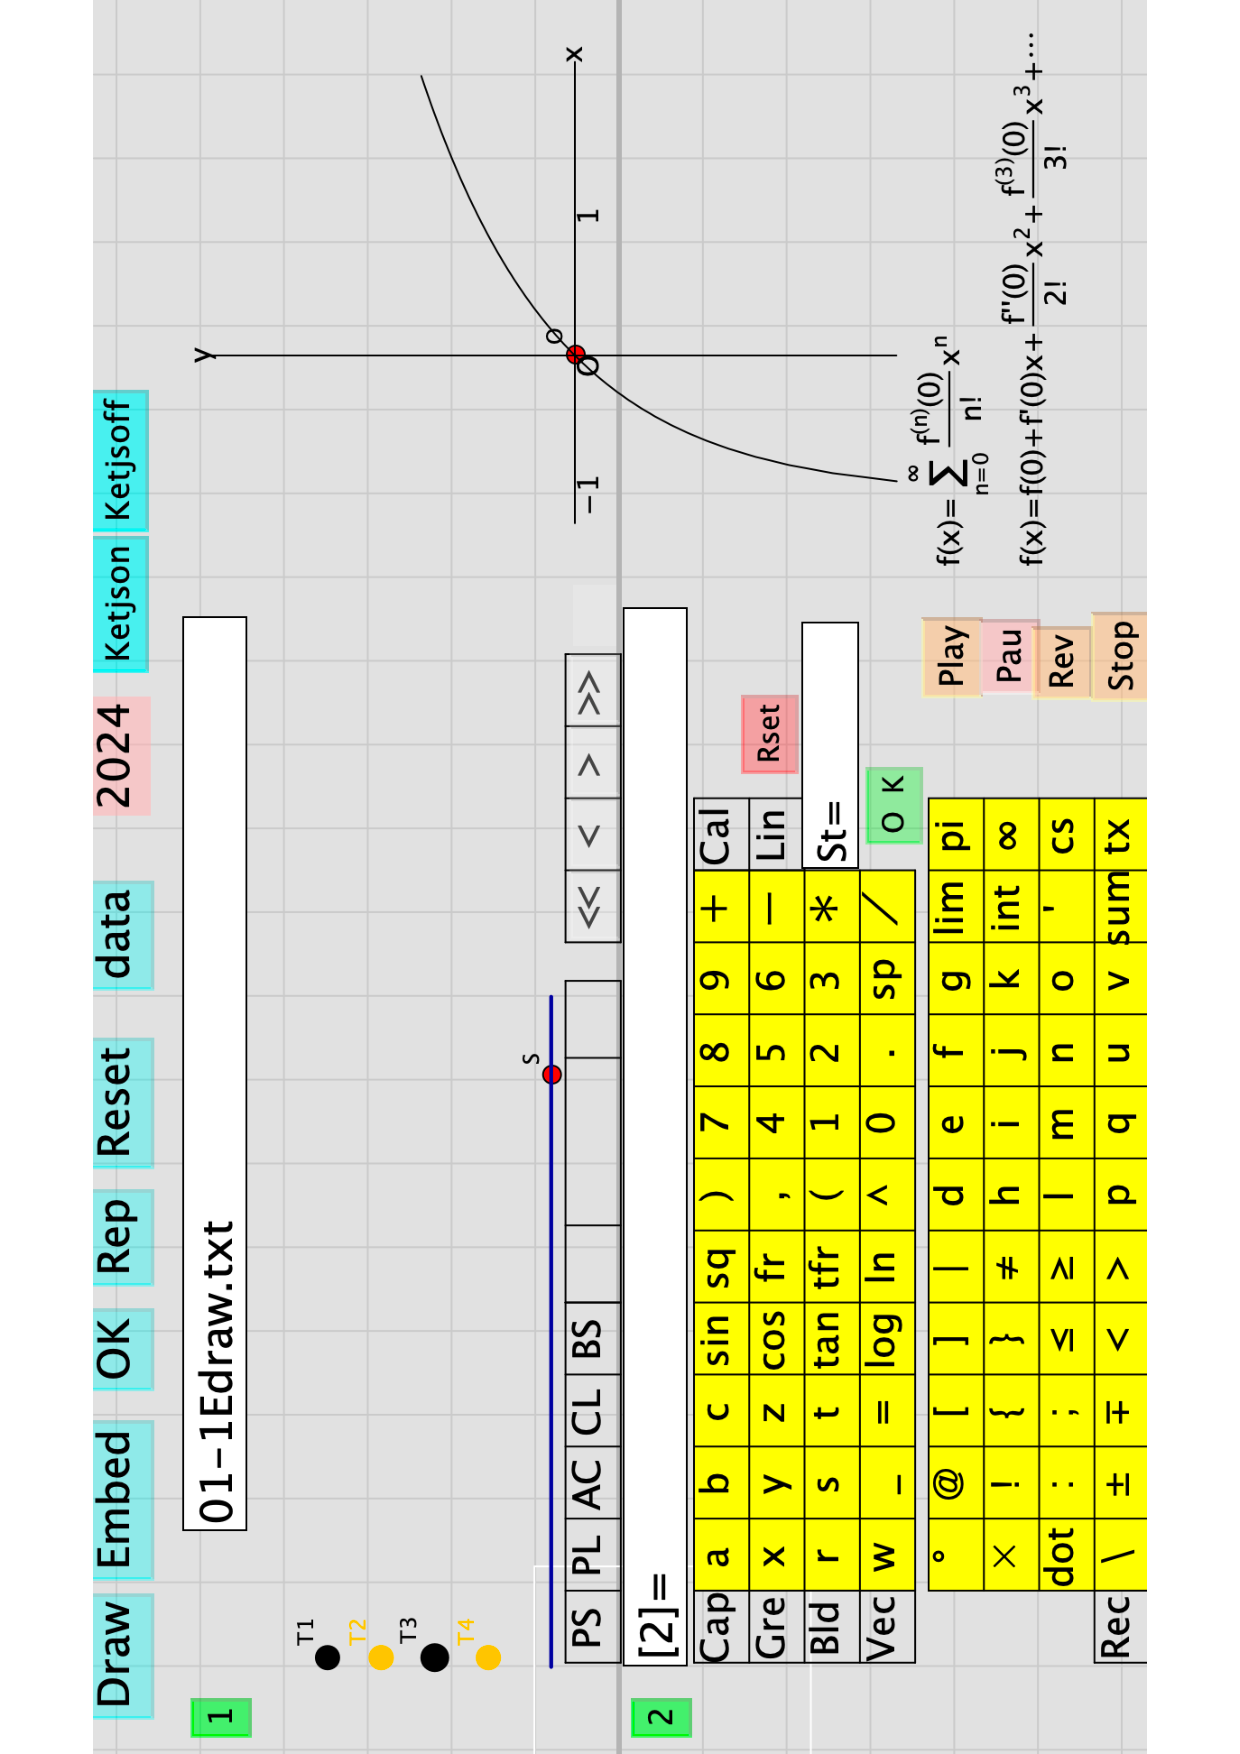
\includegraphics[bb=0.00 0.00 595.00 842.00,width=7cm,angle=-90]{fig/toolembed.pdf}}
\addtext{3}{4.}{Create an embedded file, `kettaskv01-1Ed.html',}
\addtext{8}{}{using `toolembed.cdy'.}
\end{layer}

%%%%%%%%%%%%%

%%%%%%%%%%%%%%%%%%%%

\newslide{Teaching materials}

\vspace*{18mm}

\textinit
\settext{5}{10}{110}

\begin{layer}{120}{0}
\addtext{3}{}{We have created teaching materials on the differential coefficient, titled kettaskv001-1Ed.html and kettaskv001-2Ed.html.\\
These materials consist of explanations and questions.}
\end{layer}

%%%%%%%%%%%%%

%%%%%%%%%%%%%%%%%%%%

\newslide{Teaching materials}

\vspace*{18mm}

\textinit
\settext{5}{10}{130}

\begin{layer}{120}{0}
\putnotese{-60}{-130}{
\includegraphics[bb=0.00 0.00 595.00 842.00,width=25cm]{fig/qrcode.pdf}}
\addtext{0}{}{kettaskv001-1Ed.html, kettaskv001-2Ed.html}
\end{layer}

%%%%%%%%%%%%%

%%%%%%%%%%%%%%%%%%%%

\newslide{Teaching materials}

\vspace*{18mm}

\textinit
\settext{5}{10}{110}

\begin{layer}{120}{0}
\putnotese{-15}{-82}{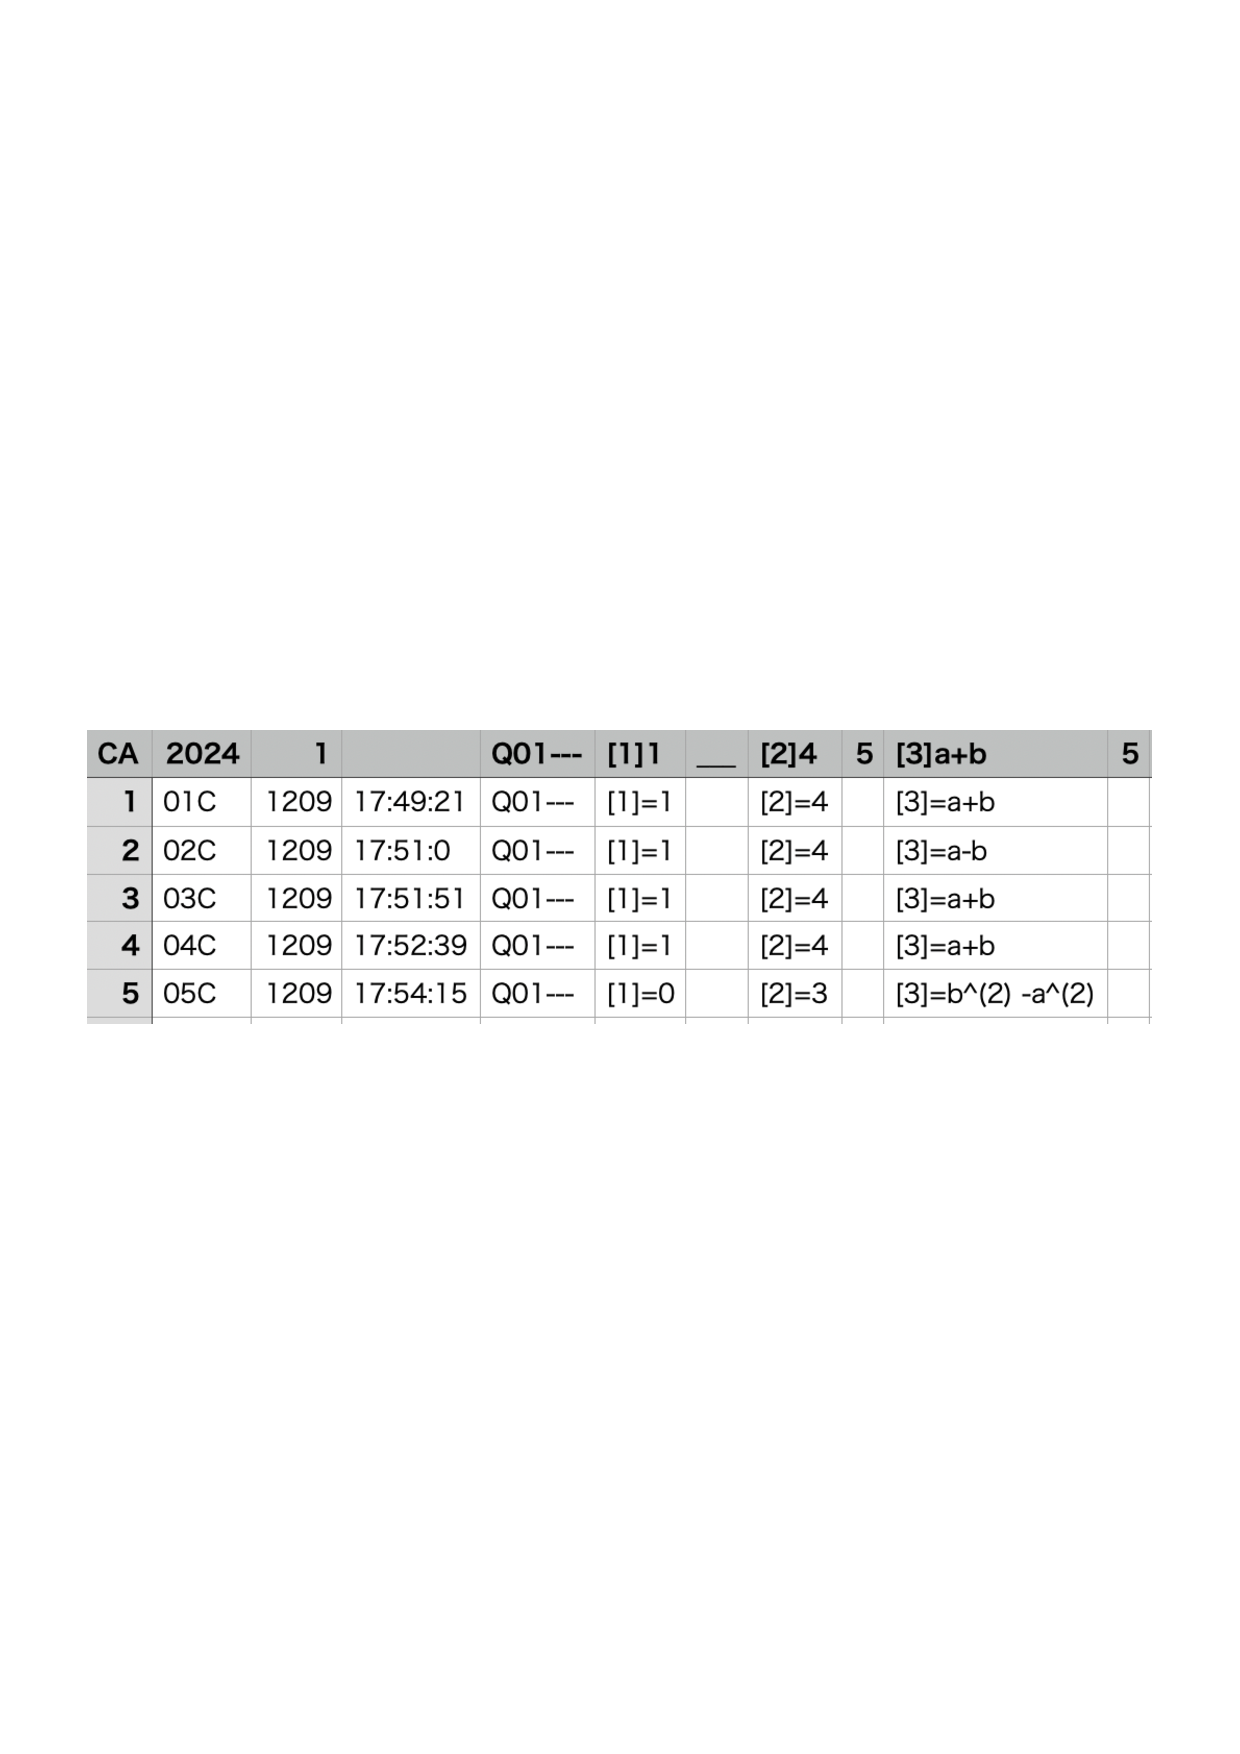
\includegraphics[bb=0.00 0.00 595.00 842.00,width=16cm]{fig/anschart.pdf}}
\addtext{18}{}{File of answers : anschart001-1.csv}
\end{layer}

%%%%%%%%%%%%%

%%%%%%%%%%%%%%%%%%%%


\sameslide

\vspace*{18mm}

\textinit
\settext{5}{10}{110}

\begin{layer}{120}{0}
\putnotese{-15}{-82}{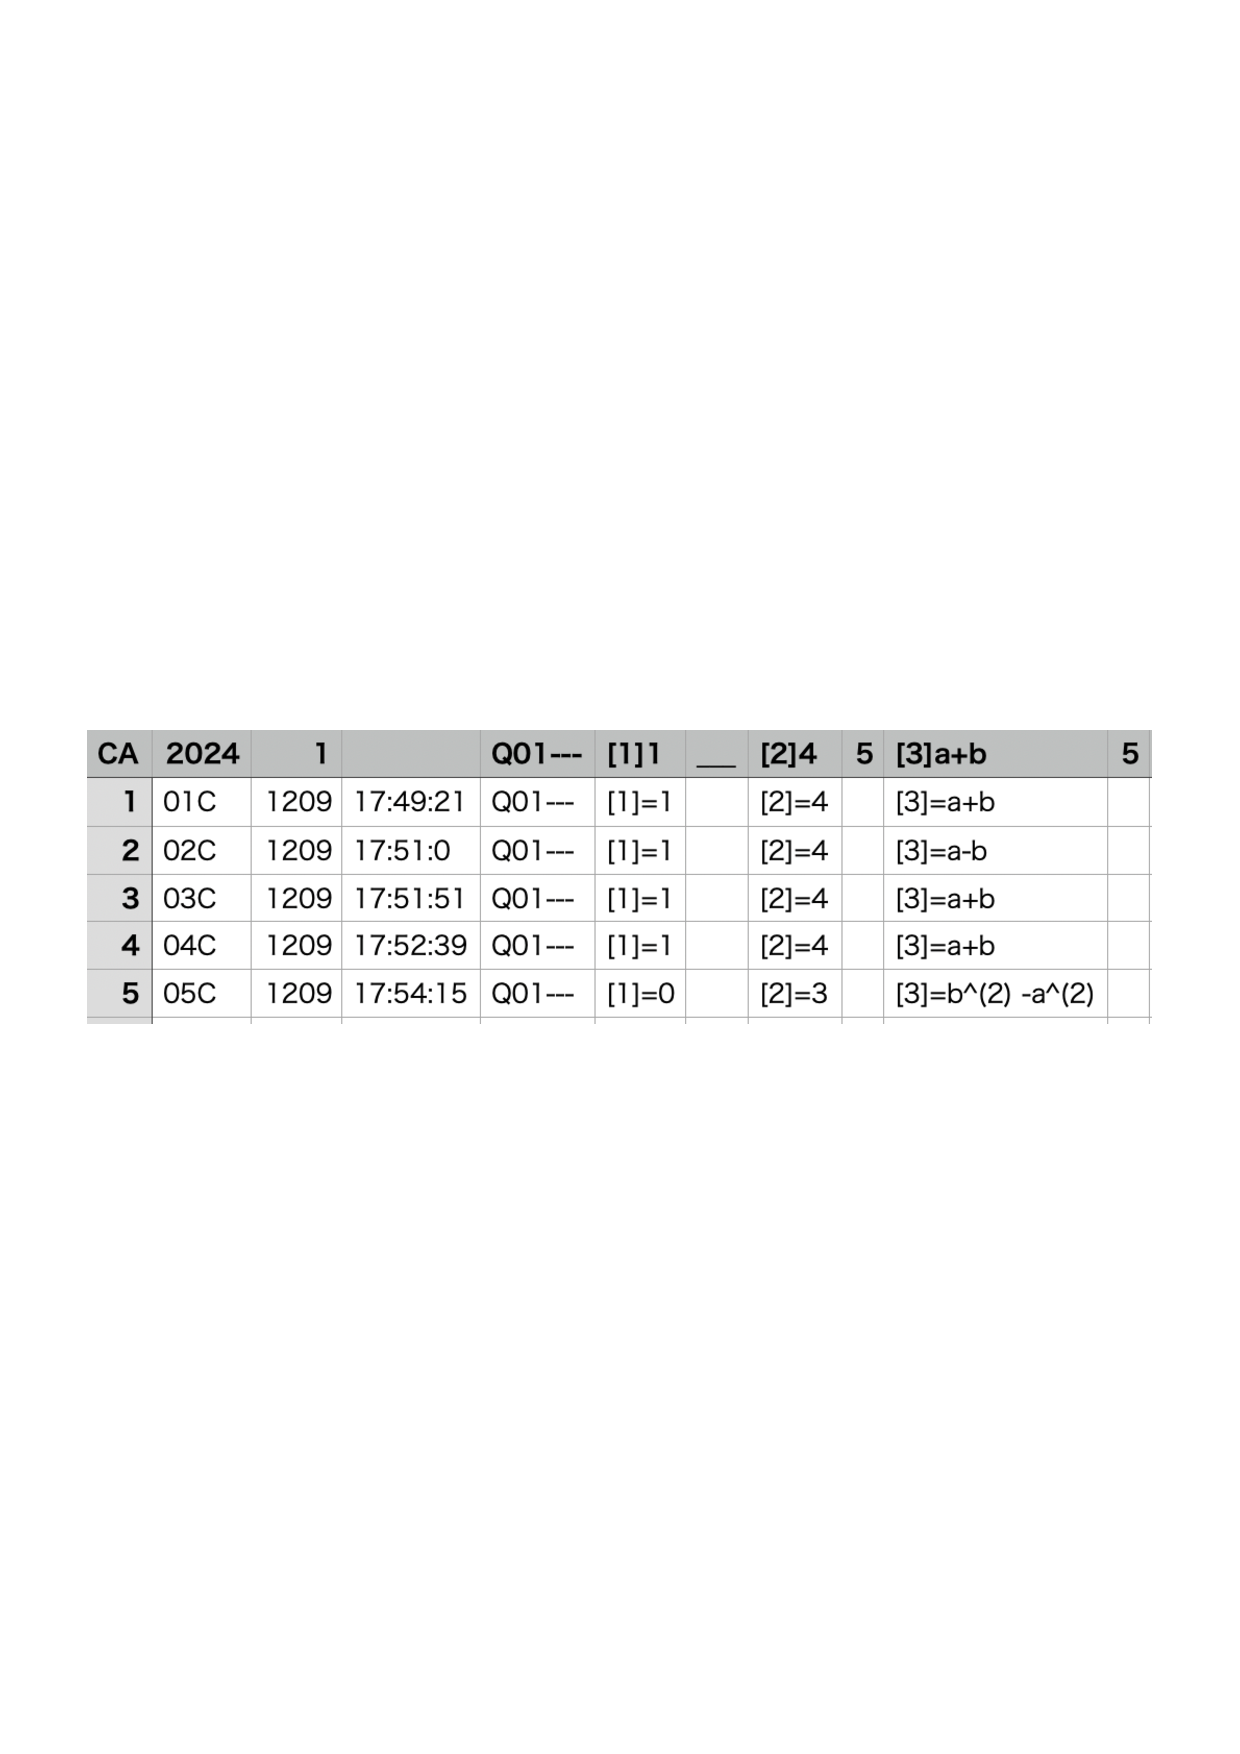
\includegraphics[bb=0.00 0.00 595.00 842.00,width=16cm]{fig/anschart.pdf}}
\addtext{18}{}{File of answers : anschart001-1.csv}
\addtext[40]{3}{}{The teacher will check the answers given by the students and then move on to the next explanation.}
\end{layer}


\newslide{Concluding remark}

\vspace*{18mm}

\textinit
\settext{5}{9}{113}

\begin{layer}{120}{0}
\addtext{3}{}{We can easily create interactive teaching materials with KeTLMS, and we will assess their effectiveness from now on.}
\end{layer}

\label{pageend}\mbox{}

\end{document}
